\documentclass[12pt, a4paper]{article}
\usepackage{graphicx}
\usepackage{array}
\usepackage[T2A]{fontenc}
\usepackage[utf8]{inputenc}
\usepackage[english,russian]{babel}
\usepackage{color}
\usepackage{listings}
\let\stdsection\section
\renewcommand\section{\newpage\stdsection}
\definecolor{lightgray}{rgb}{.9,.9,.9}
\definecolor{darkgray}{rgb}{.4,.4,.4}
\definecolor{purple}{rgb}{0.65, 0.12, 0.82}
\graphicspath{{./images/}}
\lstdefinelanguage{JavaScript}{
  keywords={typeof, new, true, false, catch, function, return, null, catch, switch, var, if, in, while, do, else, case, break},
  keywordstyle=\color{blue}\bfseries,
  ndkeywords={class, export, boolean, throw, implements, import, this},
  ndkeywordstyle=\color{darkgray}\bfseries,
  identifierstyle=\color{black},
  sensitive=false,
  comment=[l]{//},
  morecomment=[s]{/*}{*/},
  commentstyle=\color{purple}\ttfamily,
  stringstyle=\color{red}\ttfamily,
  morestring=[b]',
  morestring=[b]"
}
\lstset{
   language=JavaScript,
   backgroundcolor=\color{lightgray},
   extendedchars=true,
   basicstyle=\footnotesize\ttfamily,
   showstringspaces=false,
   showspaces=false,
   numbers=left,
   numberstyle=\footnotesize,
   numbersep=9pt,
   tabsize=2,
   breaklines=true,
   showtabs=false,
   captionpos=b
}
\author{Андрей Лушников}
\title{Разработка и реализация алгоритмов деформирования трехмерной геометрии анатомии человека на основе WebGL}
\date{Апрель 2012 год}

\begin{document}
\maketitle

\tableofcontents
\newpage

\section{Введение}
Каждый программный продукт на протяжении всех стадий жизни сопровождает много
разнообразных проблем. Это и проблемы его поддержки, и проблемы переносимости, и
проблемы контроля версий и устаревания. Эти проблемы характерны как для рядовых
программ, которые знакомы каждому пользователю, так и для специализированных
программ, используемых врачами в их ежедневной практике для оценки,
визуализирования и прогнозирования результатов пластических операций. Один из
современных подходов к распространению программного обеспечения, носящий
название ``Software as a Service'' - призван решить целый класс таких проблем.

Software-as-a-Service (далее ``SAAS'') - модель использования программного
обеспечения, при которой программный продукт выполнен в виде Web-приложения, и
разработчик самостоятельно управляет его развитием. Пользователи имеют доступ к
приложению через сеть интернет, при этом они избавлены от затрат, связанных с
установкой, обновлением и поддержкой работоспособности оборудования и
работающего на нем программного обеспечения.

В работе было решено использовать этот подход для создания средства визуализации
и изменения формы 3D моделей.  Цель выполненной работы - создать программу и веб
сервис для визуализации и изменения формы трехмерной модели с использованием
вычислений на сервере. Использование клиент-серверной системы дает возможность
перенести трудоемкие алгоритмы обработки геометрии на серверную часть,
значительно снизив требования для клиентских рабочих станций.

\section{Постановка цели}
Программное обеспечение, разработанное специально для врачей и решающее
различные медицинские задачи, зачастую обладает большим количеством недостатков.
Оно не кроссплатформенно, а его установка зачастую трудоемка. Оно предъявляет
дополнительные требования к рабочим станциям врачей, что сужает область
применения.

Основной задачей данной дипломной работы было разработать программный редактор,
позволяющий загружать и редактировать трехмерную модель, и при этом полностью
следовать модели SAAS, что избавило бы его от большого количества недостатков,
присущих программному обеспечению в общем и медицинскому программному
обеспечению в частности. Тем не менее, необходимо было дополнительно исследовать
возможность переиспользования программных модулей, написанных на С++ для
desktop-приложений редакторов геометрий, в новом редакторе.

\section{Архитектура}
\subsection{Описание архитектуры}
\subsubsection{Клиент}
Для выполнения поставленных целей было решено использовать клиент-серверную
архитектуру. В роли клиента выступает Rich Internet Application, полностью
написанное на HTML5.0 и Javascript, для отображения графики используется
перспективная технология WebGL.

WebGL - это библиотека для программного обеспечения, которая расширяет
возможности языка программирования JavaScript, позволяя ему создавать
интерактивную 3D графику внутри любого совместимого с ней веб-браузера. Код на
WebGL выполняется с помощью видеокарты. Технология
разрабатывается промышленным консорциумом Khronos Group, который
специализируется на выработке открытых стандартов интерфейсов программирования в
области создания и воспроизведения динамической графики и звука. Активное
участие в разработке и внедрении стандарта так же принимают разработчики
браузеров Apple Safari, Google Chrome, Mozilla Firefox, Opera,  а также
специалисты компаний AMD и NVidia. На данный момент технология поддерживается в
последних версиях браузеров Safari, Mozilla, Opera и Chrome, а так же в браузере
Internet Explorer вместе с плагином IEWebGL. Среди мобильных устройств данная
технология уже поддерживается в браузере аппарата Nokia N900, а так же в
браузере Safari Mobile начиная с версии операционной системы iOS 4.2
\footnote{стоит отметить, что использование WebGL разрешено в браузере Mobile
Safari только в контексте рекламных объявлений iAd}

\subsubsection{Сервер}
Cервеная часть была написана на платформе node.js. Эта технология позволяет
исполнять JavaScript на стороне сервера, причем в качестве движка используется
высокопроизводительный V8, разработанный компанией Google.

Преимущества от использования динамического слабо-типизированного
прототипно-ориентированного языка на стороне сервера заметны далеко не сразу.
Однако использование одного и того же языка на стороне клиента и сервера
позволяет переиспользовать код (например, для проверки форм) и снижает затраты
при передаче данных между клиентом и сервером, т.к. код описания модели тоже может
быть переиспользован. Серверные скрипты на JavaScript по своей природе являются
полностью асинхронными, что упрощает масштабирование серверов на Node.js.

\subsubsection{Переиспользование legacy-кода}
Для поддержания возможности переиспользования модулей и алгоритмов, написанных
на С++ в процессе работы над desktop-приложениями, используется технология
Apache Thrift. Эта технология была разработана в Facebook по аналогии с Google
Protocol Buffers и служит для написания приложений на нескольких языках
программирования. Thrift работает следующим образом: по описанной в специальном
файле и на специальном языке модели можно создать файлы описаний этих моделей
для любого из 20 языков, а по описанному на том же thrift-языке rpc-методу можно
сгенерировать thrift-сервер для интересующего языка, обрабатывающий вызов этого
метода.

\subsection{Альтернативы}
В процессе выбора технологий для решения поставленных задач было проведено исследование,
изучающее альтернативные подходы. Ниже изложены изученные альтернативные
подходы, их достоинства и недостатки.

\subsubsection{Flash на стороне пользователя}
%% В каких-каких годах? Проверить по вики!
В начале 2000х годов большую популярность снискала технология Flash,
позволяющая создавать RIA\footnote{Rich Internet Application} и
сильно оживляющая сайты. Технология остается популярной и по сей день,
однако она все больше и больше вытесняется HTML5, в который были добавлены
многие необходимые для успешной конкуренции с платформой Flash компоненты.
За счет своей огромной популярности технология обладает обширным сообществом,
большим количеством учебных материалов и даже движком для обработки и редеренга
3D-графики. Однако вместе с этими большими
преимуществами технология Flash обладает серией больших недостатков.

Во-первых, для успешной работы flash требуется установка специального плагина. Плагин
динамично развивается и обладает только свойством back-compatability
\footnote{Редкая программа обладает свойством forward-compatibility}, а потому он
становится виновником фрагментации кода.

Во-вторых, некоторое время назад компания Apple категорично отказалась от
поддержки Flash технологии на своей мобильной операционной системе iOS. Несмотря
на то, что в то время это решение вызвало ожесточенные споры, спустя некоторое
время компания Adobe свернула все работы по созданию flash-клиента под мобильную
операционную систему Android. В связи с тем, что львиная доля устройств работает
на операционных системах iOS и Android, и что поддержка технологии на этих
устройствах не запланирована, будущее Flash на мобильных устройствах
представляется туманным. По совокупности этих двух факторов технология была
отвергнута.

\subsubsection{unity вместо webGL}
Платформа Unity зарекомендовала себя в качестве мощного средства создания 2D и
3D приложений под консоли и настольные компьютеры под управлением OS X и
Windows. Платформа предоставляет возможность разрабатывать WEB-приложения с
использованием одной из следующих опций:
\begin{itemize}
    \item Использование специального Unity-плагина для браузеров
    \item Использование экспериментального движка на основе Flash
\end{itemize}
Использование технологии Unity позволяет создавать насыщенные графические сцены,
однако двустороннее взаимодействие плагина с javascript-функциями страницы для
создания полноценного RIA затруднено. Необходимость установки плагина для
пользования ресурсом и проприетарность вкупе с высокой стоймостью программы
заставили отказаться от этой технологии.

\subsubsection{Ruby on Rails вместо Express.js/node.js}
Строго говоря, сравнивать Ruby on Rails и node.js не правильно, т.к. это просто
разные вещи: Ruby on Rails - это фреймворк для создания web-приложений, а
node.js в свою очередь - библиотека для асинхронного чтения-записи. Поэтому
выбор стоял между использованием Ruby on Rails и Express.js.

С идеалогической точки зрения это очень похожие фреймворки, приспособленные для
создания и быстрого прототипирования REST-сервисов. Ruby on Rails является
более солидным и развитым проектом, нежели express.js. Однако его использование
налагает на разработчика необходимость конвертации объектов из одного языка в
другой при клиент-серверных взаимодействиях, а так же заставляет отказаться от
потенциальной возможности переиспользовать некоторые участки кода, написанные
для исполнения на стороне клиента, на стороне сервера.

Ввиду всего вышесказанного было решено использовать Express.js/node.js на
стороне сервера

\subsubsection{Protocol Buffers вместо Apache Thrift}
Для создания приложений с использованием нескольких языков встает проблема
взаимодействия модулей. Традиционным решением является абстракция удаленного
вызова процедур, когда один модуль по средствам какого-нибудь протокола кодирует
данные и передает их процедуре другого модуля на обработку. Ответ этой процедуры
кодируется с использованием того же протокола и отправляется вызывавшему.

В описанном выше взаимодействии важную роль играет сериализация и десериализация
объектов, а так же поддержание согласованности программного кода для выполнения
этих задач на каждом из языков программирования. Для решения этих задач широко
применяется одна из следующих технологий:
\begin{itemize}
    \item Google Protocol Buffers
    \item Apache Thrift
\end{itemize}

Технология Apache Thrift является в некотором роде последователем Google
Protocol Buffers, и разработана была в свете опыта использованяи последней. Сравнение двух технологий удобно отображать в виде сравнительной
таблицы.

\begin{center}
\scalebox{0.7}{%
    \begin{tabular}{ | c | c | c |}
    \hline
    & \textbf{Apache Thrift} & \textbf{Google Protocol
    Buffers} \\ \hline
    \textbf{Форматы} & Binary, JSON & Binary \\ \hline
    \textbf{Поддержка Node.js} & Включена в официальную поставку & В виде сторонних
    библиотек \\ \hline
    \textbf{Транспортный уровень} & Включен в официальную поставку & В виде сторонних
    библиотек \\ \hline
    \textbf{Документация} & Посредственная & Очень хорошая \\
    \hline
    \end{tabular}
}
\end{center}

Допольнительно стоит отметить, что быстродействие обоих фреймворков примерно
одинаково, поэтому по совокупности признаков, описанных в таблице, выбор был
сделан в пользу Apache Thrift.

\section{Детали реализации}
\subsection{Клиентские технологии}
\subsubsection{Движок для 3D графики}
WebGL - является достаточно низкоуровневой технологией, предоставляющей
пользователю возможность самостоятельно писать пиксельные и вершинные шейдеры.
Несмотря на то, что это открывает большие возможности в области создания и
обработки трехмерной графики, это достаточно трудоемкий процесс. Для
удобства и повышения скорости разработки было решено использовать популярный
движок Three.js.

Three.js содержит набор классов, написанных на языке JavaScript, которые
предоставляют высокоуровневую абстракцию над процессами создания и рендеренга
сцены. Пользователи Three.js избавлены от необходимости самостоятельно писать
шейдерные процедуры \footnote{однако такая возможность в рамках движка им
предоставляется} и могут мыслить объектами и материалами. Однако все модели
хранятся в виде javaScript-объектов, которые на каждом этапе рендеренга при
необходимости синхронизируются с буферами WebGL. Важно отметить, что все
высокоуровневые расчеты геометрии (например, пересечение луча с объектами сцены)
программируются на языке javaScript и выполняются на уровне виртуальной
JavaScript машины, а значит на прямую зависят от ее быстродействия.

\subsubsection{Инструменты для обработки графики}
В созданном приложении есть два инструмента, которыми пользователь может
взаимодействовать с объектом.
\begin{enumerate}
    \item Инструмент "Рука". Этот инструмент используется для свободного
    вращения объекта вдоль осей
    \item Инструмент "Деформация". Этот инструмент используется для изменения
    геометрии объекта
\end{enumerate}
В процессе написания приложения встала задача разработать такой код, чтобы
добавление новых инструментов в последствии было как можно более безболезненно.
Для этого было решено использовать шаблон проектирования Strategy, который
определяет семейство алгоритмов и обеспечивает их взаимозаменяемость.

В рамках приложения шаблон Strategy был применен следующим образов. Каждый
инструмент описывается классом следующего вида
\begin{lstlisting}
function FooTool(context) {
    this.context = context;
}

FooTool.prototype.setUp = function() {
    // set up event listeners for context
}

FooTool.prototype.tearDown = function() {
    // remove all set event listeners
}
\end{lstlisting}

Когда пользователь выбирает инструмент Foo, у текущего контекста вызывается метод \\
\texttt{applyMouseStrategy(FooTool)}, который написан следующим образом
\begin{lstlisting}
ManagedObject.prototype.applyMouseStrategy = function(Strategy) {
    if (this.mouseStrategy != null) {
        this.mouseStrategy.tearDown();
    }
    this.mouseStrategy = new Strategy(this);
    this.mouseStrategy.setUp();
}
\end{lstlisting}
В этом методе происходит следующая цепочка событий
\begin{enumerate}
    \item Метод проверяет, есть ли какой-нибудь действующий инструмент, и если
    есть, то вызывает у него метод \texttt{tearDown()}.
    \item Создается новый инструмент с помощью переданной в метод
    функции-конструктора класса нового инструмента, созданный объект
    присваевается внутренней переменной выбранного инструмента
    \item У нового инструмента вызывается метод \texttt{setUp()}, который
    устанавливает инструмент на контекст
\end{enumerate}

\subsubsection{Тесселляция}
На некотором этапе разработки приложения возникла потребность добавить
тесселляцию объектов.

Тесселляция - технология, с помощью которой возможно увеличить количество
многоугольников в полигональной трёхмерной модели. В процессе тесселляции
объектов, составленных целиком из треугольных полигонов \footnote{В случае
использования четырехугольных полигонов добавление новых вершин необязательно,
достаточно поделить диагональю каждый полигон пополам}, необходимо добавлять
новые вершины. В этом крылась первая проблема: объекты, загруженные в буферы
WebGL, не могут изменить количество вершин, содержащихся в их геометрии. Так как
объект загружается в буферы WebGL при первом рендеренге, то для обхода этой
проблемы нужно было либо тесселлировать объекты только один раз до
необходимого размера ребра непосредственно после загрузки и до рендеренга на
экране, либо тесселлировать объект, удалять его со сцены и пересоздавать.
Преимущество первого метода над вторым в том, что он не повлияет значительно на
скорость работы приложения, однако он не позволяет добиться динамической
тесселляции, которая становится доступной при использовании второго метода.
При разработке планировалось опробовать алгоритмы тесселляции с использованием
первого метода, а потом перейти на динамическую тесселляцию при успехе первого
этапа.

При предварительном тесселлировании объектов и их дальнейшем рендеренге была
выявлена серия проблем.

\begin{itemize}
    \item При тесселлировании простейших геометрических фигур с четырехугольыми
    гранями сбиваются цвета граней
    \item При тесселлировании загруженных *.OBJ-объектов в модели появляются
    отверстия в местах стыках граней (Рис. ~\ref{fig:holes-in-model} на странице
    ~\pageref{fig:holes-in-model})
\end{itemize}

\begin{figure}[htb]
\centering
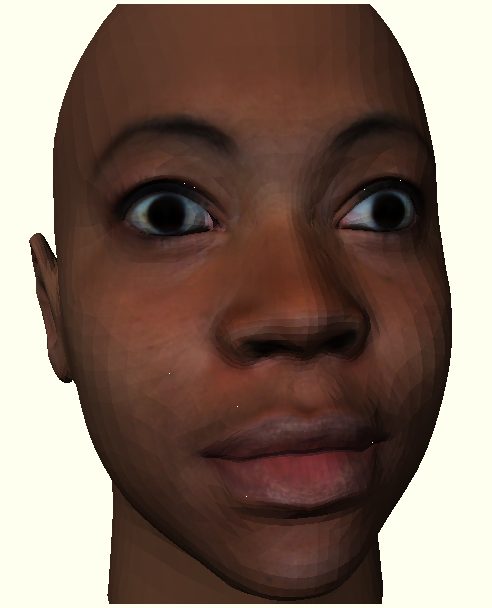
\includegraphics[width=0.8\textwidth]{holes-in-model.png}
\caption{Отверстия в модели}
\label{fig:holes-in-model}
\end{figure}

Если четырехугольные грани являются довольно редким объектов при построении
геометрии объектов, то второй недостаток существенен при работе с моделями.
Самостоятельное изучение кода тесселляции движка никаких результатов в
исправлении недостатка алгоритма не дало. В багтрекер группы разработчиков был
отправлен соответствующий отчет об ошибке, а изменения в коде приложения,
связанные с тесселляцией, были откачены назад.

\subsubsection{Проблема поворота}
Тут надо написать про проблему с поворотом объекта, про разные
координатные системы и про решение этой проблемы ввиде перемножения
матриц
\subsubsection{Шина событий}
Тут надо рассказать про EventBus, про обеспечение двунаправленных
коммуникаций между модулями приложения, а так же почему этот подход
можно считать достаточно удачным.
\subsubsection{Инструмент ``Деформация''}
Тут надо написать про инструмент деформация, рассказать про его формулы,
а так же не забыть его доделать так, чтобы он не изменял те вершины, что
находятся в другом направлении от направления деформации
\subsubsection{Использование технологии AJAX}
Тут надо написать про то, что все клиент-серверные взаимодействия сделаны по
технологии AJAX, зачем это сделано, и что, в частности, пришлось пойти на
уступки и добавить поддержку полных путей для загрузки моделей через url для
удобства. Частая ошибка, которая все ломала: относительные, а не абсолютные
адреса ссылок у действий.

\subsection{Серверные технологии}
\subsubsection{Серверная платформа node.js}
Тут надо сказать пару слов об этой платформе, почему она такая хорошая,
какие ей есть альтернативы (тут heavy wiki!)
\subsubsection{Фреймворк Express.js}
Тут надо обосновать необходимость использования серверного фреймворка,
аргументируя решением таких задач, как маршрутизация и рендеринг представлений
\subsubsection{HTML препроцессор Jade}
Тут нужно обосноват использование html-препроцессора jade, рассказать про его
достоинства и про то, почему его удобно использовать (видимо, вики)
\subsubsection{Конвертация загруженных *.obj-объектов}
Рассказать, как это делается, что происходит, какие врапперы для чего были
написаны, как и где хранятся объекты

\subsection{Серверные вычисления}
\subsubsection{Формулировка задачи}
Тут надо еще раз кратко рассказать (еще раз - потому как один раз это уже должно было
быть в ведении) про большой codebase на C++ и про необходимость как-то
интегрировать этот код
\subsubsection{Применение thrift-технологии}
Рассказать про то, что есть один файл model.thrift, что он описывает типы
данных, а так же один сервис. Можно даже скопировать частично этот файл сюда, по
крайней мере код описания сервиса так точно. Что по этому файлу генерятся стабы
для С++ и для js, а так же скелет для С++ сервера. Что этот скелет потом
с помощью скрипта-генератора наполняется содержанием на основе содержимого папки
algo, и с помощью готового makefile'а можно быстро собрать готовый
thrift-сервер.
\subsubsection{Проблема с десериализацией 8-байтного вещественного типа}
Тут надо рассказать, что у node-thrift'a была проблема с десериализацией Double,
о том что она была локализована, устранена, и соответствующий патч был послан в
сообщество на рассмотрение
\subsubsection{Организация С++ кода}
Рассказать про то, что С++ код можно писать довольно-таки обособленно,
рассказать про проблему с идентификацией алгоритмов и с решением, включающим в
себя мета-информацию в комментариях к алгоритму, которая парсится специальным
скриптом. Рассказать про специальные ruby-скрипты для пользователя и их опции

\subsection{Деплоинг приложения}
Проблема деплоинга приложения, использование сначала сбоственной машины, а потом
облачного сервиса heroku.com и его стека приложений CEDAR для временного
хостинга приложения


\section{Результат}
\subsection{Общий результат}
Сделано бла-бла-бла, можно сказать, проведен эксперимент по возможности
использования WebGL и что его можно считать удачным.
\subsection{Проведенные тесты}
\subsubsection{Тесты производительности Three.js}
Надо рассказать про некоторое количество конфузов, которые возникли при работе
с движком. Например, про то, что пересечение луча со сценой работает на уровне
JavaScript'a и потому не очень скоростное, хотя и использует отсечения по
описывающей сфере
\subsubsection{Тесты производительности node-thrift}
Рассказать про неожиданное падение в скорости при сериализации объектов в
node-thrift, о некоторых замерах времени, а так же сказать, что это очень плохо
и хотелось бы это пофиксить. Можно зафигачить какую-нибудь табличку со
сравнительными данными.
\subsection{Выводы}
\end{document}
